\documentclass[pdftex,10pt,a4paper]{article}
\usepackage{hyperref}
\usepackage{listings}
\usepackage{xyling}
\usepackage{ctable}

\input xy
\xyoption{all}

\begin{document}

  \title{SQL Windowing Functions with Hive}
  \author{Harish Butani \\
  \texttt{harish.butani@sap.com}}
  \maketitle

  \section{Overview}
This document describes a solution for issue (\cite{hive1}). Hive
allows you to define UDFs, UDAFs and UDTFs. But none of these fit the
model of Table-In/Table-Out functions needed to implement a generic
solution. Here we propose a solution that runs with Hive as opposed
to enhancing Hive. SQL Analytical functions lend themselves to being
processed as an add-on layer. By keeping the Windowing processing
outside of Hive we will be able to provide similar functionality for
Pig; we already support Native MR processing.But admittedly this
architecture misses opportunities in Query Optimization and
interoperability. Long term SQL Windowing functions should be integrated into
the Hive Engine. For now, we try to address the interoperability issue by
making it very simple syntactically to combine Hive queries with Windowing
functions. We also think this is an interesting exercise in extending
Hive; we plan to use this architecture to provide other OLAP
functionality in the future. Finally we hope that windowing functions
are useful on their own.

The Windowing Processor works with Hive in several modes: {\em Hive}
and {\em MR} are the 2 major modes. The Windowing Query is fashioned
on the Oracle Analytical clauses(\cite{odoc}). Here is a simple Windowing Query:
  {\small
   \lstset{keywordstyle=\bfseries\underbar, emphstyle=\underbar,
     language=SQL, showspaces=false, showstringspaces=false}
  \label{qry1}
   \begin{lstlisting}[caption={A simple Windowing Query},frame=shadowbox, numbers=left]
   from <select county, tract, arealand 
         from geo_header_sf1 
         where sumlev = 140>
   partition by county
   order by county, arealand desc
   with rank() as r,
        sum(arealand) over rows between 
                            unbounded preceding and 
                            current row as cum_area,
   select county, tract, arealand, r, cum_area
   where <r \\> 3>
   into path='/tmp/wout' 
   \end{lstlisting}
   }

\begin{itemize}
\item the Source of the Windowing Query can be a Hive Query or table
  among other things.
\item The Query itself provides an area to express partitioning,
  ordering and Windowing expressions
\item The output of the Query can be stored using any
  SerDe/OutputFormat combination.
\end{itemize}

In the following we first explain the Windowing Query, next we
describe how a Query is Processed, then we describe the Modes of
operation, and finally we provide some final thoughts.

  \section{The Windowing Query}
  Consider Query \ref{qry1}. The Query form is:
  \begin{itemize}
  \item the {\em tableinput} clause specifies the input of the
    Query. In this example the input is an {\em embedded Hive
      Query}. Other possibilities are a {\em Hive tableName} or a {\em
      tableinput} clause that contains all the details(location,
    SerDe, Format, columns, columnTypes etc) about the input.
  \item the {\em partition} and {\em order by} clauses specify what
    columns the rows are ordered on and what are the partition/group
    boundaries. The order by columns must be a superset of the
    partition columns.Currently the ordering is specified globally and
    not on a per function basis(this is possible to do; time/resource
    constraints is why it is not available). The Window functions are applied on each Partition.
  \item Next the Query contains a list of function
    expressions. Currently there are 16 functions available. These are
    loosely  divided into Ranking, Aggregation and Navigation
    functions. Not all functions support a windowing clause. Functions
    are described by an annotation that specifies their details: name,
    description, windowing support, args with their names, types and if they are required/optional.
  \item The Processor uses Groovy for expression support. So arguments
    to functions can be columns, literals(strings, numbers or boolean)
    and also groovy expressions. Groovy expressions are enclosed in
    $<>$. For e.g. when requesting a {\em sum} one may write it as
    $sum(arealand)$ which is saying compute the sum over the $arealand$
   column; but one can also write $sum(<arealand/2>)$, which is a sum
   over the arealand divided by 2.
  \item The window clause supports both range boundaries and value
    boundaries. Boundaries can both start and end at the Current Row.
  \item The Select List is a comma separated list of identifiers
    and/or groovy expressions. Examples of groovy expression usage are:
    expressing ratios over computed aggregations, also available are
    lead and lag functions to do relative comparisons/computations
    like compute the delta etc.
  \item the {\em where} clause can be used to filter result rows. This
    can be used to do TopN queries. As shown here the Top 3 tracts(by
    land area) for each county are listed.
  \item the {\em output} clause is used to express the location, SerDe
    and Format of the output file. At the time of writing this
    document,  we don't provide the next logical step of creating a
    Hive table that wraps the output. Its coming soon. In this example
    the defaults are used so apart from the filepath other parameters
    are optional.
  \end{itemize}
  
  A Hive mode query looks very similar, except that the tableinput
  provides the details about the Input; in this case the Windowing
  Process is spawned by the Hive Script Operator:
  {\small
   \lstset{keywordstyle=\bfseries\underbar, emphstyle=\underbar,
     language=SQL, showspaces=false, showstringspaces=false}
   \begin{lstlisting}[caption={A Hive mode Query},frame=shadowbox, numbers=left]
from tableinput(
 columns = \'p_partkey,p_name,p_mfgr,p_brand,p_type,p_size,
                   p_container,p_retailprice,p_comment\',
 \'columns.types\' = \'int,string,string,string,string,int,
                              string,double,string\' )
 partition by p_mfgr 
 order by p_mfgr, p_name 
with 
 rank() as r, 
 sum(p_size) over rows between 2 preceding 
                    and 2 following as s, 
 min(<p_size>) over rows between 2 preceding 
                    and 2 following as m[int], 
 denserank() as dr, cumedist() as cud, 
 percentrank() as pr, 
 ntile(<3>) as nt, 
 count(<p_size>) as c, 
 count(<p_size>, \'all\') as ca, 
 count(<p_size>, \'distinct\') as cd, 
 avg(<p_size>) as avg, 
 stddev(p_size) as st, 
 first_value(p_size) as fv, 
 last_value(p_size) as lv, 
 first_value(p_size, \'true\') over rows between 2 preceding 
                                    and 2 following as fv2 
 select p_mfgr,p_name, p_size, r, s, m, dr, cud, pr, nt, c, 
          ca, cd, avg, st, fv,lv, fv2
   \end{lstlisting}
   }
  
   \begin{itemize}
   \item this Query lists more functions supported: denserank, percentrank, count (with all and distinct variations), stddev, $first\_value$, $last\_value$.
   \item In hive mode quotes must be escaped; this is because of handling by ScriptOperator and/or the shell. Additionally newlines may have to be removed. See below for a complete hive query.
   \item In hive mode the Processor assumes the input stream is coming in from stdin and the format is TypedBytesSerDe.
   \end{itemize}
   
   The details of the language are beyond the scope of this doc; interested readers should look at the antlr grammar and the annotations for each function.
   
\section{Processing Details}
 The Windowing Processor is a generic Query Processor that can work in multiple modes. Conceptually it is fed a sorted input stream and a Windows Query that it generates a Output Stream that contains the results of the Windowing functions. Currently the Processor works in MR and Hive mode. We describe the Modes in the next section; here we describe the how a Query is evaluated.

\begin{figure}[h]
\centering
    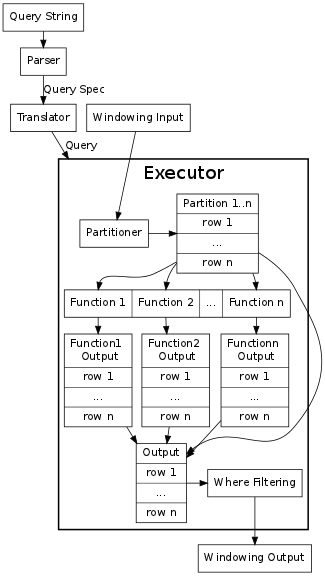
\includegraphics[scale=0.5]{query.png}
\caption{Execution of a Query}
\label{qry}
  \end{figure}
  The internal  flow of processing a Query  is shown in Figure \ref{qry}.
  \begin{itemize}
  \item A Query String is converted into a Query Object and passed to
    the Executor. A Query contains a list of Windowing Functions, the
    Windowing Input and the Windowing Output.
  \item The Executor streams the rows from the WindowingInput through
    the Partitioner. This produces a table for each Partition. It then
    passes the table to each Windowing Function which evaluates the
    function for the Partition ( and if necessary for a specific
    window for each row in the partition). The function outputs an
    Object that provides the context in which the where Clause
    expression and the Select List are evaluated.
  \item The Executor then creates an Output Object for each input row
   in the partition by processing the Select List. Before this the
   where clause filter is applied, if present and only those rows that
   meet the criteria are output. The Output Object  is then passed to
   the Windowing Output.
  \item during execution the Functions and the Output processing have
    a GroovyShell at their disposal. When functions evaluate Groovy
    Expressions the columns of the Input are bound to the execution
    environment and can be used as variables. When the Output is
    processed both the input columns and the outputs of functions are available as variables.
  \item The {\em Windowing Input} is responsible for making Writables
    available to the processing environment. The specific process of
    how this happens depend on the Mode of Operation. Details are
    beyond this introductory doc. See \cite{wndwi} for details.
  \end{itemize}

\section{Modes of Operation}
\subsection{MapReduce Mode}
\begin{itemize}
\item In this mode the WindowingProcessor assumes it can interact with
  a HiveMetaStoreServer and with a Map-Reduce cluster.
\item Further it assumes it can access a service that can execute {\em
    embedded Hive Queries}. Hence there are 2 variations of this mode:
  \begin{description}
    \item[Windowing CLI:] In this mode the User interacts with a CLI
      client that is literally an extension of the Hive CLI. The
      WindowingProcessor runs inside a sandbox in this landscape but
      asks the Hive CLI to execute Hive Queries. We describe this mode
      in detail below.
    \item[Hive ThriftServer:] In this setup the WindowingProcessor
      connects to hive via the Thrift interface. We use this in our
      MRTest environment. This mode is useful for embedding the
      WIndowing jar in your application.
  \end{description}
\item In this mode the Windowing Processing is done in a MR job. The
  Processor setups up the Job with the relevant partitioning, sorting
  configuration. The Windowing functions are run in the Rduce Job. The
  details of the Job are outside the scope of this doc. See
  \cite{wndwi} for details.
\end{itemize}

\subsubsection{MapReduce Mode using the Windowing CLI}
We provide a CLI interface. This is exposed as a hive service and is
invoked as '$hive --service windowingCli -w <path to windoing jar>$'. In
this interface users can enter hive or windowing queries. The {\em
  wmode} settings controls how a command is interpreted. See Figure \ref{mrarch}.
for the overall architecture.
\begin{figure}[h]
\centering
    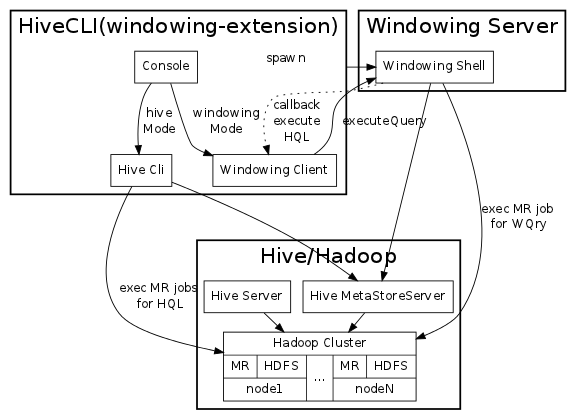
\includegraphics[scale=0.5]{mrarch.png}
\caption{Overall Architecture: MR mode}
\label{mrarch}
  \end{figure}

\subsection{Hive Mode}
The overall flow of processing is shown in Figure \ref{hivearch}. Processing involves streaming data from a Hive Query/Table via the Script Operator:
\begin{figure}[h]
\centering
    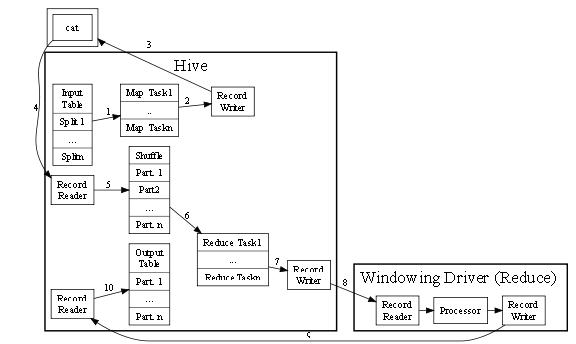
\includegraphics[scale=0.5]{architecture.jpg}
\caption{Hive Mode: Overall processing of a Windowing Request}
\label{hivearch}
  \end{figure}
\begin{itemize}
\item The Map Operation is a Noop. It is used so that the M-R shuffle mechanism gets invoked for partitioning and sorting the input rows.
\item The {\em Readers} and {\em Writers}  capture the transformations that have to happen to integrate with an external process. The Windowing Process uses the TypedBytesSerDe for transforming bytes to Objects and back. The readers and writers handle the transformations from the input SerDe to TypedBytesSerDe and then to the output SerDe.
\item The Windowing Process is invoked during the Reduce phase. The Window process assumes that the data being streamed in is sorted. The Window process takes a {\em Windowing Query} that lists the operations to perform on the input stream.
\item The Output from the Windowing process is streamed back to the Script Operator. After going through the RecordReader it can then flow into the next operation in the Hive Query Graph.
\end{itemize}
In Hive mode the Windowing Query is expressed as a Script Operation. Here is a complete Query in Hive mode:
{\small
   \lstset{keywordstyle=\bfseries\underbar, emphstyle=\underbar,
     language=SQL, showspaces=false, showstringspaces=false}
   \begin{lstlisting}[caption={A complete Query in Hive Mode},frame=shadowbox, numbers=left]
CREATE TABLE windowing_test as
select p_mfgr,p_name, p_size, r, s, m, dr, cud, pr, nt, c, 
         ca, cd, avg, st, fv,lv, fv2
from
(
from (
  from part
  select transform(p_partkey,p_name,p_mfgr,p_brand,p_type,
                             p_size,p_container,p_retailprice,p_comment)
    ROW FORMAT SERDE 'org.apache.hadoop....TypedBytesSerDe'
    RECORDWRITER 'org.apache.hadoop.hive....TypedBytesRecordWriter'
    USING '/bin/cat'
    as (p_partkey,p_name,p_mfgr,p_brand,p_type,p_size,
         p_container,p_retailprice,p_comment)
    ROW FORMAT SERDE 'org.apache.hadoop...TypedBytesSerDe'
    RECORDREADER 'org.apache.hadoop....TypedBytesRecordReader'
    DISTRIBUTE BY p_mfgr
    SORT BY p_mfgr, p_name
) map_output
  select transform(p_partkey,p_name,p_mfgr,p_brand,p_type,
                p_size,p_container,p_retailprice,p_comment)
    ROW FORMAT SERDE 'org.apache.hadoop....TypedBytesSerDe'
    RECORDWRITER 'org.apache.hadoop....TypedBytesRecordWriter'
    USING 'java 
       -cp "antlr-runtime-3.4.jar:windowing.jar:groovy-all-1.8.0.jar...." 
       windowing.WindowingDriver 
       -m hive 
        -q "from tableinput(
        columns = \'p_partkey,p_name,p_mfgr,..\', 
        \'columns.types\' = \'int,string,string,...\' ) 
        partition by p_mfgr 
        order by p_mfgr, p_name 
        with
  	rank() as r,
 	 sum(p_size) over rows between unbounded preceding 
 	                              and current row as s,
 	 ntile(<3>) as nt,
select p_mfgr,p_name, p_size, r, s, nt"'
as (p_mfgr,p_name, p_size, r, s, nt)
ROW FORMAT SERDE 'org.apache.hadoop....TypedBytesSerDe'
RECORDREADER 'org.apache.hadoop....TypedBytesRecordReader'
) reduce_output;
   \end{lstlisting}
   }


\section{Summary}
\begin{enumerate}
\item As an analogy to Oracle, look at this as a quick implementation in PL/SQL. Typically new DB features are implemented in PL/SQL, once they show value they are pushed down into the Engine and finally integrated with the Semantic layers.
\item In this regard it would have been helpful if there was an In-Process Script Operator. This would avoid the overhead of streaming data to an external process.
\item The implementation hopefully shows a technique for providing extensible mini DSLs. We hope to use this pattern for introducing other Operations specifically for dimensional processing in OLAP.
\end{enumerate}

\section{Possible Next Steps}
\begin{description}
\item[Performance]  In Hive Mode the data is going through several transformations: serialization through TypedBytesSerDe, inter process streaming, copy to a Standard Java Object, serialization through TypedBytesSerDe, and finally inter process streaming. Need to look at avoiding some of these conversions. Along these lines it would be nice to avoid streaming data through to an external process. In MR mode the transformation to Standard Java Object can be eliminated.

Another performance improvement is on the evaluation of the Functions.  Also, currently the Executor is very simple. It can be parallelized, and it can be made smarter when computing windows. Currently for computing windows the Executor computes the raw expressions for each row in the Partition in the first pass and then processes each row w.r.t. to its window range in a second pass. In this way it avoids computing the raw expressions multiple times, but it still takes $O(n^2)$  time.
\item[Multiple Orderings] currently we only support a single Ordering; whereas in SQL each function can have its own ordering.  This is fairly easy to support by reordering a partition before evaluating the function.
\item[Multiple Partitioning] In SQL each function can have its own partitioning.  Instead of providing partitioning specification per function, an initial step would be to allow for multiple Partitioning clauses.  This is a fairly involved process and would be done only if there is significant demand for it.

\end{description}
  
  \begin{thebibliography}{Dillon 83}
   \bibitem[Hadoop]{hdop} Hadoop website {\em http://tiny.cc/b72fb}
   \bibitem[Hive]{hive} Hive website {\em http://tiny.cc/559sh}
   \bibitem[Hive ICDE]{hv10} Hive - A Petabyte Scale Data Warehouse Using Hadoop {\em http://tiny.cc/o5q6h}
   \bibitem[Hive 896]{hive1} Hive Issue 896 {\em
       https://issues.apache.org/jira/browse/HIVE-896}
   \bibitem[Wndw Interal Doc.]{wndwi} SQL Windowing development details:
     posted on website.
     \bibitem[Oracle Doc.]{odoc} Oracle SQL Reference: SQL for Analysis and Reporting http://tinyurl.com/7s9qgjr
  \end{thebibliography}
\end{document}
